\documentclass[10pt,oneside,swedish]{lips}

%\usepackage[square]{natbib}\bibliographystyle{plainnat}\setcitestyle{numbers}
\usepackage[round]{natbib}\bibliographystyle{plainnat}

% Configure the document
\title{Kravspecifikation}
\author{Redaktörs namn}
\date{1 november 2015}
\version{1.0}

\reviewed{Ewa, Karl}{2015-xx-xx}
\approved{Moa}{2015-xx-xx}

\projecttitle{Inspirerande titel}

\groupname{Projektgrupp}
\groupemail{groupmail@liu.se}
\groupwww{http://www.liu.se/grouppage}

\coursecode{TSRT10}
\coursename{Reglerteknisk projektkurs}

\orderer{Beställare, Linköpings universitet}
\ordererphone{+46 xxxxxx}
\ordereremail{bestallare@liu.se}

\customer{Kund, Företag X}
\customerphone{+46 xxxxxx}
\customeremail{kund@foretagx.com}

\courseresponsible{Boss Person}
\courseresponsiblephone{+46 xxxxxx}
\courseresponsibleemail{the.boss@liu.se}

\supervisor{Handledare}
\supervisorphone{+46 xxxxxx}
\supervisoremail{hand.ledare@liu.se}

\smalllogo{logo} % Page header logo, filename
\biglogo{logo} % Front page logo, filename

\cfoot{\thepage}
\begin{document}
\maketitle

\cleardoublepage
\makeprojectid

\begin{center}
  \Large Projektdeltagare
\end{center}
\begin{center}
  \begin{tabular}{|l|l|l|}
    \hline
    \textbf{Namn} & \textbf{Ansvar} & \textbf{E-post}\\
    \hline
    Anna Andersson & kundansvarig (KUN) & Annan111@student.liu.se\\
    \hline
    Beata Bson & dokumentansvarig (DOK) & Beabs222@student.liu.se\\
    \hline
    Cecilia Cson & designansvarig (DES) & Ceccs333@student.liu.se\\
    \hline
    Doris Dson & testansvarig (TEST) & Dords444@student.liu.se\\
    \hline
    Erik Eson & kvalitetssamordnare (QA) & Eries555@student.liu.se\\
    \hline
    Fredrik Fson & implementationsansvarig (IMP) & Frefs666@student.liu.se\\
    \hline
    Greta Gson & Projektledare (PL) & Gregs777@student.liu.se\\
    \hline
  \end{tabular}
\end{center}

\cleardoublepage
\tableofcontents

\cleardoublepage
\section*{Dokumenthistorik}
\begin{tabular}{p{.06\textwidth}|p{.1\textwidth}|p{.45\textwidth}|p{.13\textwidth}|p{.13\textwidth}} 
  \multicolumn{1}{c}{\bfseries Version} & 
  \multicolumn{1}{|c}{\bfseries Datum} & 
  \multicolumn{1}{|c}{\bfseries Utförda ändringar} & 
  \multicolumn{1}{|c}{\bfseries Utförda av} & 
  \multicolumn{1}{|c}{\bfseries Granskad}\\
  \hline
  \hline
  1.0 & 2015-11-25 & Första versionen & X &    \\
  \hline
  0.2 & 2015-11-20 & Andra utkast & Y &    \\
  \hline
  0.1 & 2015-11-18 & Första utkast & Z &    \\
  \hline
\end{tabular}

\cleardoublepage
\pagenumbering{arabic}\cfoot{\thepage}

\section{Inledning}
\label{sec:inledning}

Text
\begin{figure}[htbp]
  \centering
  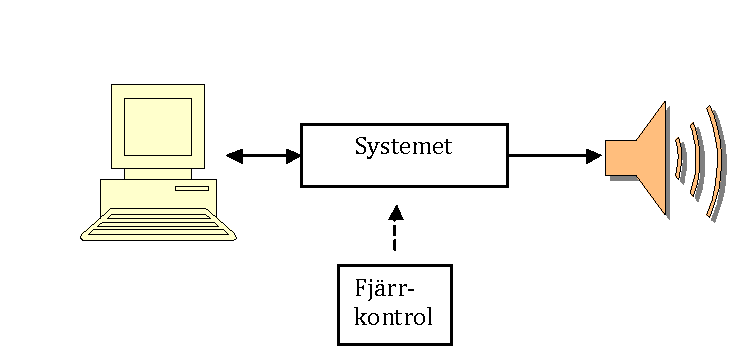
\includegraphics[width=.7\textwidth]{sys}
  \caption{Systemet i dess omgivning}
  \label{fig:sys}
\end{figure}

\begin{requirements}
  \requirementno & Alla dokument skall uppfylla instruktioner
  beskrivna i \citep{spraknamnd:2000} & 1\\
\end{requirements}

\subsection{Parter}
Text

\subsection{Syfte och mål}
Text

\subsection{Användning}
Text

\subsection{Bakgrundsinformation}
Text

\subsection{Definitioner}
Text

\section{Översikt av systemet}
Text
\begin{figure}[htbp]
  \centering
  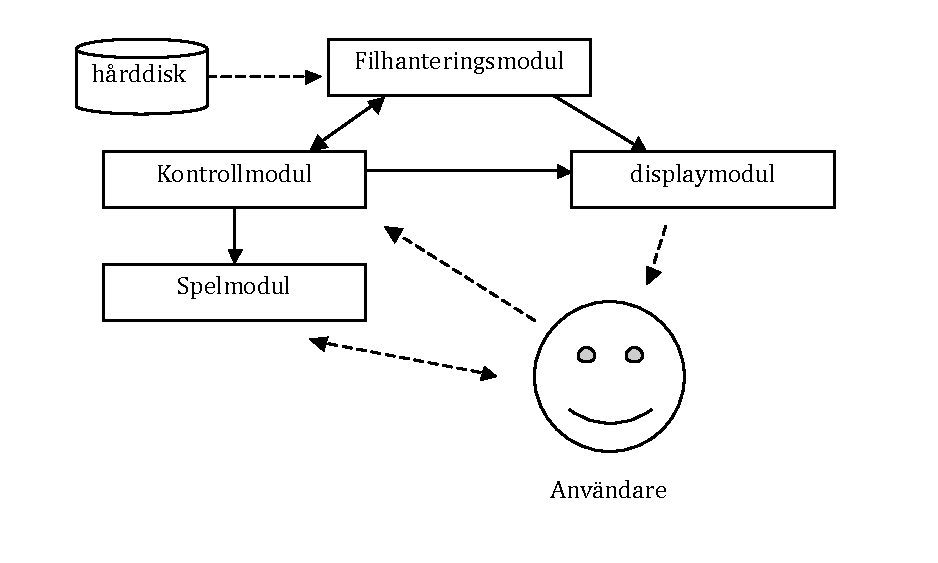
\includegraphics[width=.7\textwidth]{outline}
  \caption{En översikt av systemet}
  \label{fig:oversikt}
\end{figure}

\subsection{Grov beskrivning av produkten}
Text

\subsection{Produktkomponenter}
Text

\subsection{Beroenden till andra system}
Text

\subsection{Ingående delsystem}
Text

\subsection{Avgränsningar}
Text

\subsection{Designfilosofi}
Text

\section{Delsystem 1}
Text
\begin{figure}[htbp]
  \centering
  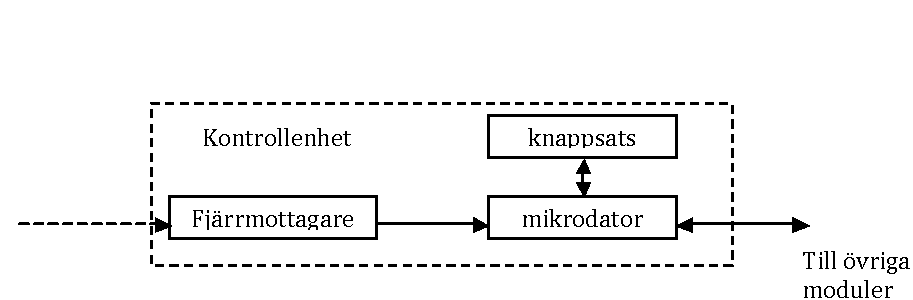
\includegraphics[width=.7\textwidth]{delsys1}
  \caption{Delsystem 1}
  \label{fig:delsys1}
\end{figure}

\subsection{Inledande beskrivning}
Text
\begin{requirements}
  \requirementno & Felmeddelanden skall vara på svenska & 1\\
\end{requirements}

\subsection{Gränssnitt}
\begin{requirements}
  \requirementno\label{req:r2} & Kravtext & Utgått\\
  \ref{req:r2}A & Ändring av krav \ref{req:r2} & 1\\
\end{requirements}
Text

\subsection{Designkrav}
Text
\begin{requirements}
  \requirementno & Kravtext & 2\\
  \requirementno & Kravtext & 3\\
\end{requirements}

\subsection{Funktionella krav}
Text
\begin{requirements}
  \requirementno & Kravtext & 2\\
  \requirementno & Kravtext & 3\\
\end{requirements}

\section{Delsystem 2}
Text
\begin{figure}[htbp]
  \centering
  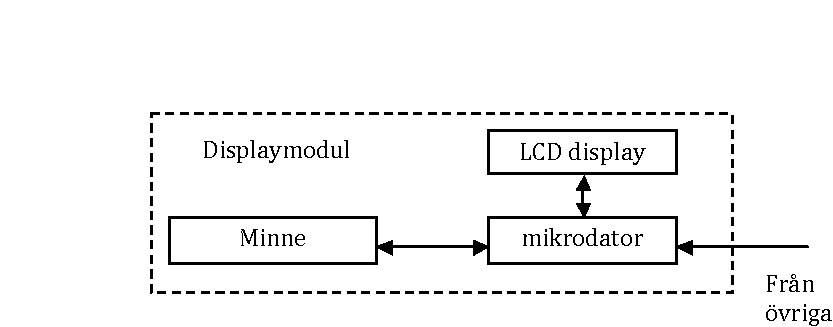
\includegraphics[width=.7\textwidth]{delsys2}
  \caption{Delsystem 2}
  \label{fig:delsys2}
\end{figure}


\subsection{Externa gränssnitt}
Text
\begin{requirements}
\requirementno & Kravtext & Bas\\  
\end{requirements}

\subsection{Designkrav}
Text
\begin{requirements}
\requirementno & Kravtext för designkrav & Bas\\
\end{requirements}


\subsection{Funktionella krav}
Text
\begin{requirements}
  \requirementno & Kravtext & Bas\\
  \requirementno & Mera krav & 	Extra\\
\end{requirements}

\subsection{Användargränssnitt}
Text
\begin{requirements}
  \requirementno & Mera krav & Bas\\
\end{requirements}

\section{Prestandakrav}
Text
\begin{requirements}
  \requirementno & Kravtext & Bas\\
\end{requirements}

\section{Krav på vidareutveckling}
Text
\begin{requirements}
  \requirementno & Kravtext & Bas\\
\end{requirements}

\section{Tillförlitlighet}
Text
\begin{requirements}
  \requirementno & Kravtext & Bas\\
\end{requirements}

\section{Ekonomi} 
Text
\begin{requirements}
  \requirementno & Kravtext & Bas\\
\end{requirements}

\section{Krav på säkerhet}
Text
\begin{requirements}
  \requirementno & Kravtext & Bas\\
\end{requirements}

\section{Leveranskrav och delleveranser} 
Text
\begin{requirements}
  \requirementno & Kravtext & Bas\\
\end{requirements}

\section{Dokumentation} 
Tabell~\ref{tab:doks} listar de dokument som skall produceras
\begin{table}[htbp]
  \centering
  \caption{Dokument som skall produceras}
  \label{tab:doks}
  \begin{tabular}{|l|l|l|l|l|}
    \hline
    Dokument & Språk & Syfte & Målgrupp & Format\\
    \hline
    Projektplan &&&&\\
    Kravspecifikation &&&&\\
    Designspecifikation &&&&\\
    Mötesprotokoll &&&&\\
    Teknisk dokumentation &&&&\\
    Efterstudie &&&&\\
    \hline
  \end{tabular}  
\end{table}

\begin{requirements}
  \requirementno & Kravtext & Bas\\
\end{requirements}

\section{Utbildning}
Text
\begin{requirements}
  \requirementno & Kravtext & Bas\\
\end{requirements}

\section{Kvalitetskrav}
Text
\begin{requirements}
  \requirementno & Kravtext & Bas\\
\end{requirements}

\section{Underhållsbarhet}
Text
\begin{requirements}
  \requirementno & Kravtext & Bas\\
\end{requirements}


\clearpage
\bibliography{references}

\cleardoublepage
\appendix

\section{Appendixtitel}

\subsection{Den första rubriken}
Text

\subsubsection{Första underrubriken}
Text

\subsubsection{Andra underrubriken}
Text

\subsubsection{Tredje underrubriken}
Text

\end{document}

%%% Local Variables:
%%% mode: latex
%%% TeX-master: t
%%% End:
